\subsection{Estimote}

Beacons are used for indoor location in this project. Estimote is one of many vendors of iBeacons. Common use cases for beacons include monitoring if the user enters a specific region of an area. This can be used to push location specific information or advertisement when a user is near a shop or even a certain product in that shop.

Estimote not only focus on typical use cases for beacons like entering a specific region, but have also specialized in indoor location of users using the beacon technology. The company developed the Estimote Indoor Location application for iOS\footnote{https://itunes.apple.com/us/app/estimote-indoor-location/id963704810} which is meant to ease configuration needed for indoor location. A user will install the beacons in a room by placing one beacon on each wall. Next the user walks along the perimeter of the room and thereby registering the location of the beacons by collecting signal strengths from the beacons and data from the phones accelerometer and/or gyroscope.
After the configuration, the application has estimated the length of and placement of walls allong with the signal strengths of each beacon.

During our tests we found that the approach for configuring the indoor locationing describe above works terribly or not at all. After configurin the room, the application would show an illustration of the registered room and we found the measurements to to be very inaccurate. The Estimote Indoor Location application was therefore abandoned for configuring a room.

\subsubsection{Configuring Rooms Programmatically}

Estimote provides Estimote Indoor Location SDK\footnote{https://github.com/Estimote/iOS-Indoor-SDK} to perform indoor locationing using beacons on iOS. The SDK provides two mechanisms for configuring a room for indoor positioning.

\begin{enumerate}
\item Using the built-in controller. The component presents the user with a guided configuration similar to the one used in the Estimote Indoor Location application.
\item Programmatically using the \texttt{ESTLocationBuilder} class.
\end{enumerate}

The built-in controller was abandoned as it uses the exact same technology as the Estimote Indoor Location application and therefore results in poor accuracy.

The \texttt{ESTLocationBuilder} lets developers configure a room programmatically by passing XY-points and an orientation to the builder. The X and Y value of each point is measured in meters. Therefore a point $(0, 0$) to $(0, 5)$ represents a horisontal line of five meters and the set of points $\{(0,0),(0,5),(5,5),(5,0)\}$ represents a room of size 5 meters by 5 meters.

\begin{listing}
\begin{swiftcode}
        let locationBuilder = ESTLocationBuilder()
        locationBuilder.setLocationBoundaryPoints([
            ESTPoint(x: 0.cmToMeter(), y: 0.cmToMeter()),
            ESTPoint(x: 537.cmToMeter(), y: 0.cmToMeter()),
            ESTPoint(x: 537.cmToMeter(), y: 60.cmToMeter()),
            ESTPoint(x: 690.cmToMeter(), y: 60.cmToMeter()),
            ESTPoint(x: 690.cmToMeter(), y: 385.cmToMeter()),
            ESTPoint(x: 0.cmToMeter(), y: 385.cmToMeter()),
        ])
        
        let ice3 = "dec18deac0c5"
        let blueberry3 = "f13173ad3185"
        let ice2 = "d470d26d33f3"
        let mint3 = "e6d39dee79c9"
        
        locationBuilder.addBeaconIdentifiedByMac(blueberry3, atBoundarySegmentIndex: 0, inDistance: 422.cmToMeter(), fromSide: .RightSide)
        locationBuilder.addBeaconIdentifiedByMac(ice3, atBoundarySegmentIndex: 3, inDistance: 222.cmToMeter(), fromSide: .RightSide)
        locationBuilder.addBeaconIdentifiedByMac(mint3, atBoundarySegmentIndex: 4, inDistance: 335.cmToMeter(), fromSide: .LeftSide)
        locationBuilder.addBeaconIdentifiedByMac(ice2, atBoundarySegmentIndex: 5, inDistance: 165.cmToMeter(), fromSide: .LeftSide)
        locationBuilder.setLocationOrientation(130)
        locationBuilder.setLocationName("Gros Stue")
        
        let location = locationBuilder.build()
\end{swiftcode}
\caption{Example usage of the \texttt{ESTLocationBuilder} class.}
\label{lst:estlocationbuilder}
\end{listing}

Listing \ref{lst:estlocationbuilder} shows how we used the \texttt{ESTLocationBuilder} to create a model of a real world living room. The resulting model is illustrated in figure \ref{fig:estlocationbuilder-livingroom}.

The builder is configured with six points that gives information about the shape of the room. Next, the beacons are added to the walls of the room. Beacons are added with the identifier of the beacon. Lastly the orientation of the room relative to north and the name of the room is set. When the room has been configured it can be stored on the users Estimote account using the Estimote SDK.

\begin{figure}
\centering
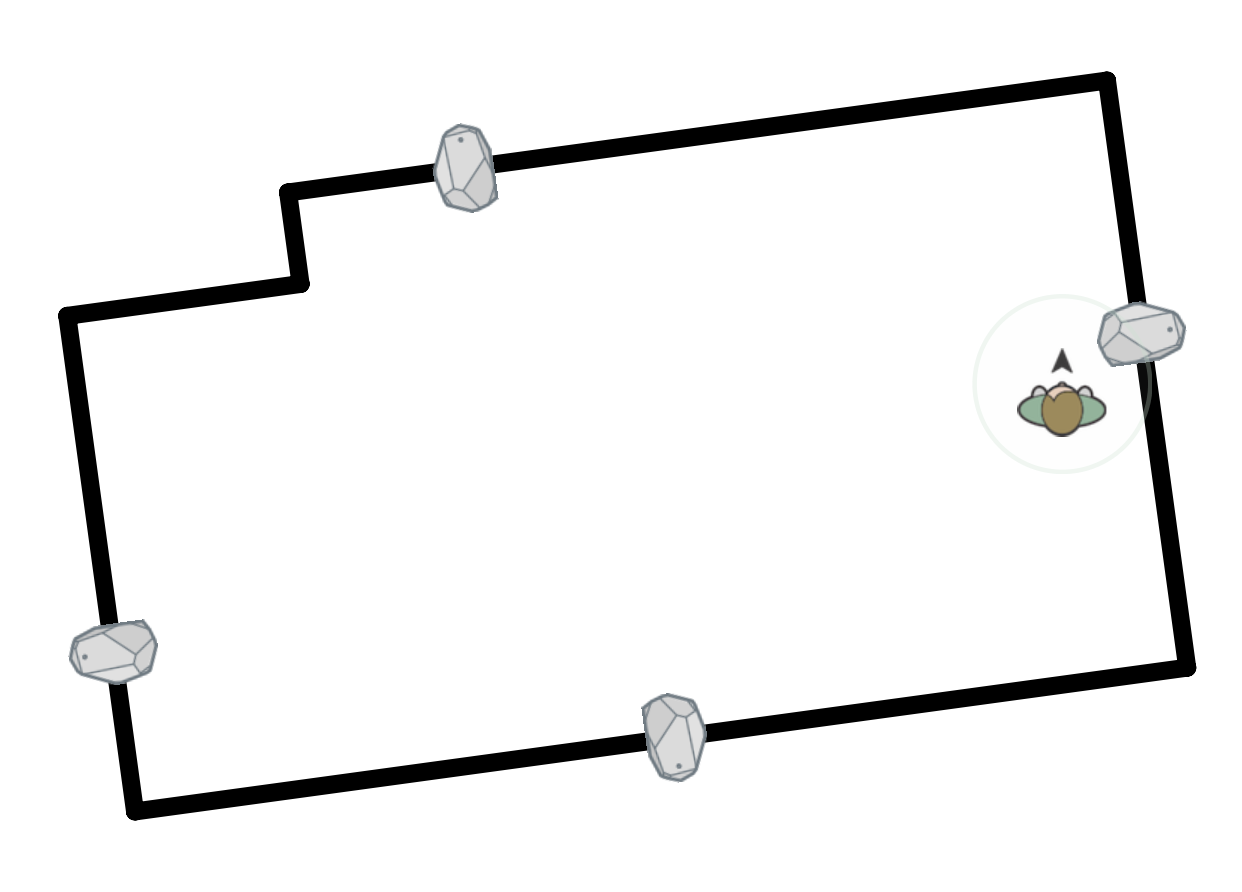
\includegraphics[width=0.33\textwidth]{images/living-room}
\caption{Model created using the \texttt{ESTLocationBuilder} as shown in listing \ref{lst:estlocationbuilder}.}
\label{fig:estlocationbuilder-livingroom}
\end{figure}

%%% Local Variables:
%%% mode: latex
%%% TeX-master: "../../master"
%%% TeX-command-extra-options: "-shell-escape"
%%% End:
